\noindent

\includegraphics[height=1.25cm]{images/pictograms/replication}
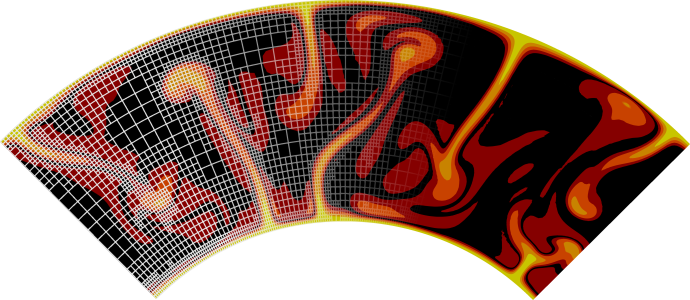
\includegraphics[height=1.25cm]{images/pictograms/aspect_logo}

\includegraphics[height=1.25cm]{images/pictograms/benchmark}

\includegraphics[height=1.25cm]{images/pictograms/under_construction}
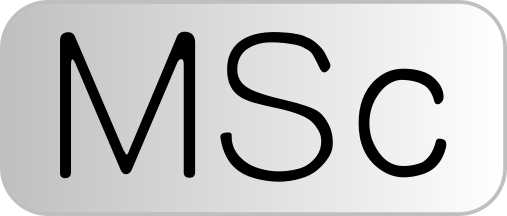
\includegraphics[height=1.25cm]{images/pictograms/msc}

\includegraphics[height=1.25cm]{images/pictograms/FEM}
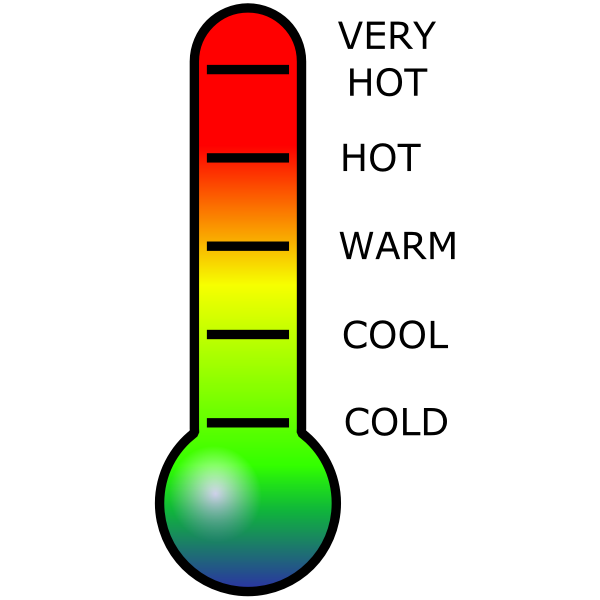
\includegraphics[height=1.25cm]{images/pictograms/temperature}

\includegraphics[height=1.25cm]{images/pictograms/paraview}

%%%%%%%%%%%%%%%%%%%%%%%%%%%%%%%%%%%%%%%%%%%%%%%%%%%%%%%%%%%%%%%%%%%%%%%%%%%%%%%%%%%%%%%%%%%%%%%%%%%

\begin{flushright} {\tiny {\color{gray} python\_codes/fieldstone\_184/text.tex}} \end{flushright}

%\lstinputlisting[language=bash,basicstyle=\small]{python_codes/template_keywords.key}

\par\noindent\rule{\textwidth}{0.4pt}

\begin{center}
\infortran
{\small Code: \url{https://github.com/cedrict/fieldstone/tree/master/python_codes/fieldstone_184}}
\end{center}

\par\noindent\rule{\textwidth}{0.4pt}

{\sl This stone was developed in collaboration with T. Weir}. 

\par\noindent\rule{\textwidth}{0.4pt}

Last revision: Jan. 20th, 2025.

\par\noindent\rule{\textwidth}{0.4pt}

%%%%%%%%%%%%%%%%%%%%%%%%%%%%%%%%%%%%%%%%%%%%%%%%%%%%%%%%%%%%%%%%%%%%%%%%%%%%%%%%%%%%%%%%%%%%%%%%%%%

This \stone is the result of the so-called Guided Research\footnote{A form of short MSc thesis at the UU.}
project by Tom Weir.
It is based on the Fortran code SimpleFEM, which is in essence an ancestor of the early FieldStone codes.

This code relies on the infamous $Q_1\times P_0$ pair. It is only 2d and isothermal.
It implements 6 analytical benchmarks. For all of them the domain is the unit square.



\begin{itemize}
\item {\tt ibench=-1}
\begin{verbatim}
uth = x**2 * (1.d0-x)**2 * (2.d0*y - 6.d0*y**2 + 4*y**3)
vth = -y**2 * (1.d0-y)**2 * (2.d0*x - 6.d0*x**2 + 4*x**3)
pth = x*(1.d0-x)-1.d0/6.d0
rho=1
gx = ( (12.d0-24.d0*y)*x**4 + (-24.d0+48.d0*y)*x**3 + (-48.d0*y+72.d0*y**2-48.d0*y**3+12.d0)*x**2 &
   + (-2.d0+24.d0*y-72.d0*y**2+48.d0*y**3)*x + 1.d0-4.d0*y+12.d0*y**2-8.d0*y**3 )
gy= ( (8.d0-48.d0*y+48.d0*y**2)*x**3 + (-12.d0+72.d0*y-72*y**2)*x**2 + & 
    (4.d0-24.d0*y+48.d0*y**2-48.d0*y**3+24.d0*y**4)*x - 12.d0*y**2 + 24.d0*y**3 -12.d0*y**4)
\end{verbatim}
\item {\tt ibench=1}
\begin{verbatim}
2D Cartesian Linear
uth = 1.d0/x 
vth = 1.d0/y
pth = -4.d0/(3.d0*x**2) - 4.d0/(3.d0*y**2) + x**2/2.d0 + y**2/2.d0  -1.d0
rho=x*y
gx=1.d0/y
gy=1.d0/x
\end{verbatim}
\item {\tt ibench=2}
\begin{verbatim}
2D Cartesian Sinusoidal
uth = 1.d0/cos(x)
vth = 1.d0/cos(y)
pth = 4.d0*sin(x)/(3.d0*cos(x)**2)+4.d0*sin(y)/(3.d0*cos(y)**2) + sin(x) + sin(y) - 3.18834
rho = cos(x)*cos(y)
gx = 1.d0/cos(y)
gy=1.d0/cos(x)
\end{verbatim}
\item {\tt ibench=3}
\begin{verbatim}
1D Cartesian Linear
uth = 1.d0/x
vth=0.d0
pth =  -4.d0/(3.d0*x**2) - x**2/2.d0 + 11.d0/6.d0
rho=x
gx=-1.d0
gy=0.d0
\end{verbatim}
\item {\tt ibench=4}
\begin{verbatim}
Arie van den Berg
uth=1.d0-x
vth=0.d0
pth = 10.d0*log(x-1) +290.9 
rho = 1.d0/(1.d0-x)
gx=10.d0
gy=0.d0
\end{verbatim}
\item {\tt ibench=5}
\begin{verbatim}
1D Cartesian Sinusoidal
uth = 1.d0/cos(x)
vth=0.d0
pth = 4.d0*sin(x)/(3.d0*cos(x)**2) - sin(x) -0.674723
rho=cos(x)
gx=-1.d0
gy=0.d0
\end{verbatim}
\end{itemize}

$\vec{h}_{el}$ is given by $\rho^{-1} \vec\upnu \cdot \vec\nabla \rho$.
The {\tt approach} parameter is a switch and it only affects how $\vec{h}_{el}$ is computed:
\begin{itemize}
\item {\tt approach=1}:
Analytical functions for $\rho,\partial_x\rho,\partial_y\rho$ are used for each quadrature point:
\begin{verbatim}
hel(1)=hel(1)+1.d0/rho(xq,yq,ibench)*(uq*drhodx(xq,yq,ibench) 
                                    + vq*drhody(xq,yq,ibench))*wq*jcob
\end{verbatim}
\item {\tt approach=2}:
Basis functions and their derivatives are used to estimate $\rho,\partial_x\rho,\partial_y\rho$ on each quadrature point:
\begin{verbatim}
hel(1)=hel(1)+1.d0/rhoq*(uq*drhodxq+vq*drhodyq)*wq*jcob 
\end{verbatim}
\end{itemize}








